The Virtual Reality System Layer is focused on delivering real-time video and tracking of the head movement on the virtual reality headset. This system contains the stereo display subsystem and the head tracking subsystem. Both of the subsystems make it possible to communicate with the Processing System Layer.

\begin{figure}[h!]
	\centering
 	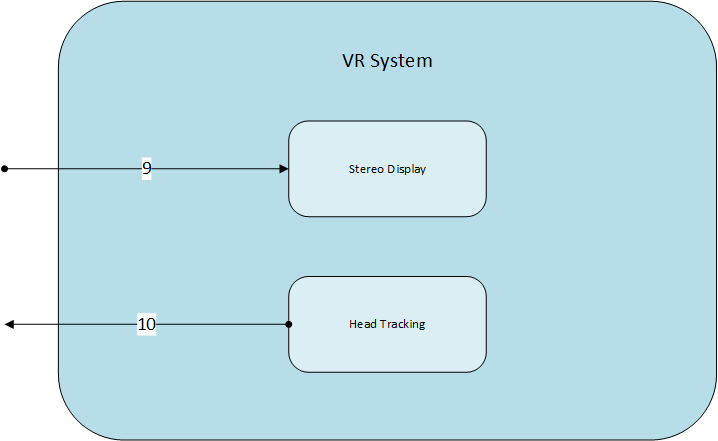
\includegraphics[width=0.75\textwidth]{images/vrsubsystem}
 \caption{Virtual Reality System Layer Subsystem Description Diagram}
\end{figure}

\subsection{Stereo Display Subsystem}
This subsystem interacts with the video output subsystem of the Processing System Layer by receiving the processed video data.

\subsubsection{Assumptions}
None

\subsubsection{Responsibilities}
The processed video data received from the Processing System Layer will be displayed through the user's virtual reality headset.

\subsubsection{Subsystem Interfaces}

\begin {table}[H]
\caption {Stereo Display Subsystem interfaces} 
\begin{center}
    \begin{tabular}{ | p{1cm} | p{6cm} | p{3cm} | p{3cm} |}
    \hline ID & Description & Inputs & Outputs \\ \hline
    \#11 & Processing System - Video Output Subsystem & \pbox{3cm}{Processed video data} & \pbox{3cm}{N/A}  \\ \hline
    \end{tabular}
\end{center}
\end{table}

\subsection{Head Tracking Subsystem}
This subsystem interacts with the gimbal controller subsystem of the Processing System Layer by sending head tracking data.

\subsubsection{Assumptions}
The accelerometer signals can be extracted from the headset. The accelerometer signals extracted from the headset can be decoded into standard PWM signals to control motor movement.

\subsubsection{Responsibilities}
Head tracking angles are taken from the user's virtual reality headset. The raw angular data will be sent to the gimbal controller subsystem of the Processing System Layer.

\subsubsection{Subsystem Interfaces}

\begin {table}[H]
\caption {Head Tracking Subsystem interfaces} 
\begin{center}
    \begin{tabular}{ | p{1cm} | p{6cm} | p{3cm} | p{3cm} |}
    \hline ID & Description & Inputs & Outputs \\ \hline
    \#12 & Processing System - Gimbal Controller Subsystem & \pbox{3cm}{N/A} & \pbox{3cm}{Raw head tracking angles}  \\ \hline
    \end{tabular}
\end{center}
\end{table}